\cotefile{69}
\scanpage{104}
\diagram{\begin{tikzcd}[ampersand replacement=\&,row sep=1ex,column sep=1em]
 \& \unsure{G|C} \&\\
 \& \deleted{\unsure{g}}\Psi(C)\arrow[u]\arrow[dl]\arrow[dr] \&\\
 G \& \& G
\end{tikzcd}}

\diagram{\begin{tikzcd}[ampersand replacement=\&,column sep=1em,row sep=.5em]
 \& P\quad a_0\;\overline{r},\overline{\pi},\overline{r'} \&\\
 \& {\underset{\gamma_0}{\Gamma}}\arrow[u]\arrow[dl]\arrow[dr] \&\\
 {\underset{c_0}{R}} \& \& {Q\quad b_0\;\widetilde{r'}\;\widetilde{r''}\;\widetilde{\sigma}}
 \arrow[from=1-2,to=3-3,dash,end anchor=north,start anchor=east]
\end{tikzcd}}

\[
\left.
\begin{gathered}
 \deleted{\unsure{\rho}}\\
 \deleted{\unsure{r,r',r''}}\\[-2pt]
 \deleted{\unsure{\pi\;\sigma}}\\
 \deleted{(rr')r''}
\end{gathered}\right\}
\begin{gathered}
 \overbrace{\overbrace{r,r'}^{\pi},r''}^{\rho}\\[-2pt]
 \underbrace{\phantom{r,}r',r''}_{\sigma}\\[-2pt]
 \underbrace{\phantom{r,r',r''}}_{\unsure{\tau|\iota}}
\end{gathered}
\qquad
\deleted{r(r'r'')}
\]
\[
\begin{array}{ccc|l}
\deleted{\unsure{a_0,b_0}}&&&\\
\deleted{(\overline{r},b_0,r)}&(\overline{\pi},b_0,\pi)&(\overline{r'},b_0,r')&\\
(a_0,\widetilde{r'},r')&\deleted{(a_0,\widetilde{r''},r'')}&\deleted{\unsure{a_0,r''}}\inserted{(a_0},\widetilde{\sigma},\sigma)&\Rightarrow\\
(\overline{r},\widetilde{r'},\pi)&\tikz[baseline=(v.base)]{\node[inner sep=2pt](v){$(\overline{\pi},\widetilde{r''},\rho)$};\draw (v.center) ellipse[x radius=2.8em,y radius=1.2em];\draw[overlay] (v.east)..controls +(0,-1.5em) and +(-1em,-1.2em)..++(13em,.15em);}&(\overline{r'},\widetilde{r''},\sigma)&(\overline{r},\widetilde{\sigma},\rho)\Leftrightarrow
\end{array}
\]
% The tail joins the oval to the right extremity of this line.
\[
\begin{aligned}
&a_0,\overline{r'},\overline{r},\overline{\pi}\\
&b_0,\widetilde{r'},\widetilde{r''},\widetilde{\sigma}\\[3pt]
&r,r',r'',\pi,\sigma,\rho
\end{aligned}
\]
\diagram{\begin{tikzcd}[ampersand replacement=\&,row sep=.65em,column sep=.6em]
 \overline{r}\arrow[d] \& \widetilde{r'}\arrow[d] \& \overline{\pi}\arrow[ddll,bend left=15]
 \& \widetilde{r''}\arrow[d] \& \overline{r'}\arrow[d] \& \widetilde{\sigma}\arrow[ddll,bend left=22]\\
 (r) \& (r')\arrow[rrr,leftrightarrow,yshift=1.2ex] \& \& (\unsure{r'|r''}) \& (r') \&\\
 \pi \& \rho \& \& \sigma \& \&
\end{tikzcd}}
\[
\begin{array}{ll}
\alpha_1=a_0 & \alpha_2=\overline{r}\\
\beta_2=\widetilde{r'} & \beta_1=\widetilde{\sigma}\\
\gamma_2=r' & \gamma_1=\sigma
\end{array}
\]
\[
\begin{aligned}
&\underline{a_0},\underline{\overline{r}},\underline{\overline{\pi}},\underline{\overline{r'}}\\
&\underline{b_0},\underline{\widetilde{r'}}\;\widetilde{r''}\;\deleted{\unsure{b}}\widetilde{\sigma}\\
&\underline{r'},\underline{\pi},\underline{\sigma},\underline{\rho}
\end{aligned}
\]
\diagram{\(\displaystyle
\left\{\begin{array}{c|c|c|c|c|c}
 \overline{\pi}&\overline{r'}&a_0&a_0&\overline{r}&\overline{r'}\\
 b_0&b_0&\widetilde{r'}&\widetilde{\sigma}&\widetilde{r'}&\widetilde{r''}\\
 \pi&r'&\multicolumn{2}{c|}{\underline{r'\hspace{1.2em}\sigma}}&\underline{\pi}&\sigma
\end{array}\right\}
\deleted{\unsure{\ne}}\;
\left\{\left(\begin{array}{c}\overline{\pi}\\\widetilde{r''}\\\rho\end{array}\right)
\deleted{\unsure{\Rightarrow}}\;\left(\begin{array}{c}\overline{r}\\\widetilde{\sigma}\\\underline{\rho}\end{array}\right)\right\}
\)}
% A continuous underline joins the r' and sigma entries of columns 3 and 4.
\[
 a_0,b_0,\overline{r},\underset{\deleted{\unsure{r''}}}{\widetilde{r''}},\overline{r'},\deleted{\unsure{\widetilde{r'}}}
 \ \bigg|\ \overset{\widetilde{r'},r'}{\overbrace{\pi,\sigma}},\rho,\overline{\pi},\widetilde{\sigma}
\]
\diagram{\begin{tikzcd}[ampersand replacement=\&,column sep=.25em,row sep=.5em]
 \& \& \& \& \& \phantom{\rho}\arrow[dddd,bend left=45]\\[-1.2em]
 {\forall\ \begin{gathered} a_0,\overline{r},\overline{r'}\in P\\ b_0,\widetilde{r''}\in Q\end{gathered}}
 \& \exists \& {\begin{gathered}\deleted{\unsure{r',\overline{\pi}\in Q}}\\\deleted{\unsure{r',\pi,\sigma,\rho}}\end{gathered}}
 \& {\begin{gathered}\overline{\pi}\in P\\ \widetilde{r'},\widetilde{\sigma}\in Q\\r',\pi,\sigma,\rho\in R\end{gathered}}
 \& \text{tels que l'on ait} \&\\
 \&\&\&\&\&\\ \&\&\&\&\&\\ \&\&\&\&\&\phantom{\rho}
\end{tikzcd}}
\diagram{\(\displaystyle
\begin{array}{cccc}
 \unsure{\overline{a_{0}}|\overline{\alpha_0}}&&&\\[-4pt]\Vert&&&\\
 \alpha_1&\alpha_2&\alpha_3&\alpha_4\\
 \beta_1&\beta_2&\beta_3&\beta_4\\
 \gamma_1&\gamma_2&\gamma_3&\gamma_4
\end{array}\qquad
\begin{array}{cccccccc}
 \alpha_1&\alpha_1&\alpha_2&\alpha_2&\alpha_3&\alpha_3&\alpha_4&\alpha_4\\
 \beta_1&\beta_2&\beta_1&\beta_2&&&&\\
 \gamma_1&\gamma_2&\gamma_3&\gamma_4&&&&
\end{array}
\)}
% archive sheet number: 105
\scanpage{106}
\[
 \dim E_7=133\quad(126\ \text{\unsure{racines}})
\]
\[
\left.\begin{array}{llll}
 x_i\quad y_{i} &1\le i\le7&14&\\
 x_{ih}&1\le i<h\le7&21&x_{ih}=-x_{hi}\\
 y_{ih}&1\le i<h\le7&21&y_{ih}=-y_{hi}
\end{array}\right\}\quad56\ \text{\unsure{indéterminé|indéterminés|indéterminées}}
\]
\[
\begin{aligned}
 &\sum_{i,j,\unsure{k|h|h,k}=1}^{7}\deleted{\sum}x_i y_j\unsure{a_{ih}|x_{ih}}y_{jh}
 +\tfrac14\sum_{\lambda,\mu,\nu,\rho=1}^{7}x_{\lambda\mu}x_{\nu\rho}y_{\mu\nu}y_{\lambda\rho}
 \unsure{+|\ast}\sum\bigl(\underline{x_i y_{\lambda\mu}y_{\nu\rho}y_{\sigma\tau}}\\[-2pt]
 &\hspace{22em}{}+y_i x_{\lambda\mu}x_{\nu\rho}x_{\sigma\tau}\bigr)
\end{aligned}
\]
\[
 \left\{\begin{gathered}
 i,\lambda,\mu,\nu,\rho,\sigma,\tau\quad\text{permutations}\\
 \text{paires de }[1,7]
 \end{gathered}\right.
\]
\[
\unsure{\mathscr L|\mathcal L|\mathfrak L}\quad\text{---}\quad \operatorname{End} V_{56}
\qquad
\underline{\sum(x_i\,dy_i-y_i\,dx_i)+
 \sum_{i,h=1}^{7}(x_{ih}\,dy_{ih}-y_{ih}\,dx_{ih})}
\]
\[
\begin{aligned}
 &\unsure{8|g|\mathfrak g}\quad\text{---}\\
 &12
\end{aligned}
\]
% archive sheet number: 107
\scanpage{108}
\(G\) groupe comm.

\(P_1\ P_2\ P_3\) trois \(G\) torseurs, \(\quad s:G\times G\times G\longrightarrow G\quad\) \unsure{appl.|l'appl.} somme
\[
 P_1\times P_2\times P_3\supset \Gamma\qquad\text{un sous-torseur sous }\operatorname{Ker}s
\]
[correspondant à une trivialisation \(\unsure{\Gamma_1|P_1}\wedge \Gamma_2\wedge \Gamma_3\overset{t}{\simeq}\mathbb{1}_{\unsure{\mathrm{TORS}(G)|\mathrm{Tors}(G)}}\)]

On va montrer que le foncteur
\[
 \{G,P_1,P_2,P_3,t\}\longrightarrow(P_1,P_2,P_3,\Gamma)
\]
\unsure{allant} des systèmes d'un \unsure{gpe|groupe} \inserted{G}, \(3\) tors. \inserted{P_i} sous \(G\) et une trivialisation \(t\) de leur produit de \unsure{Baer}, vers les quadruplets de \(3\) ens. \(P_1,P_2,P_3\) et d'une partie \(\Gamma\) de \(P_1\times P_2\times P_3\), est pl. fidèle.

Notons \(p_i:\Gamma\unsure{\relbar\joinrel\relbar|\longrightarrow} P_i,\quad p_{ij}:\Gamma\relbar\joinrel\relbar P_{ij}\quad(i\ne j)\)

(1) \uline{Les} \(p_{ij}\) \uline{sont des iso}

Se donner \((P_1,P_2,P_3\deleted{\unsure{;\Gamma}})\deleted{\unsure{\longrightarrow}}\) et \(\Gamma\subset P_1\times P_2\times P_3\) satisfaisant (1), \unsure{revient|veut} : se donner
\[
 P_1\times P_2\xrightarrow{\pi_3}P_3
\]
satisfaisant :
\[
 \left\{\begin{aligned}
 \forall\,x_1\in P_1,\quad x_2&\longmapsto \pi_3(x_1,x_2)& P_2&\xrightarrow{\sim}P_3\\
 \forall\,\unsure{x_2|x_3}\in P_2,\quad x_1&\longmapsto \pi_3(x_1,x_2)& P_1&\xrightarrow{\sim}P_3
 \end{aligned}\right.
\]
On trouve ainsi
\[
 P_1\xrightarrow{\unsure{\varphi_{123}|\varphi_{1\,23}|h_{23}}}\operatorname{Isom}(P_2,P_3)
\]
et de \(=\)
\[
 P_1\overset{\varphi_{132}}{\relbar\joinrel\relbar}\operatorname{Isom}(P_3,P_2)
\]
déduit des \unsure{précédts|précédents|précédent} par symétrie
% archive sheet number: 109
\scanpage{109}
\[
 u,\alpha,\beta
\]
\[
\begin{aligned}
 &(u,1,1,1)(\deleted{\unsure{\alpha}}1,\deleted{\unsure{\beta}}\alpha,\beta,\unsure{\gamma|\sigma})\inserted{(u^{-1},1,1,1)}
 =(u,u(\alpha),u(\beta),u(\gamma))(u^{-1},1,1,1)\\
 &(1,\alpha,\beta,\gamma)\,(\text{---}\\[-2pt]
 &\hspace{9em}=(\deleted{\unsure{u}}1,u(\alpha),u(\beta),\deleted{\unsure{u}}u(\gamma))
\end{aligned}
\]
\[
\begin{aligned}
 \operatorname{Aut}(G)\mathbin{.}(G\times G\times G)&\longrightarrow
 \unsure{\mathscr G_G|\mathcal G_G|\mathfrak S_G}\times\mathscr G_{\unsure{G|C}}\times\mathscr G_G\\
 (u,\alpha,\beta,\gamma)&\unsure{\longmapsto|\relbar\joinrel\relbar}(\tau_{\unsure{\rho|\beta}}\tau'_{\unsure{\beta|\gamma}}u,\tau_\gamma\tau'_\alpha u,\tau_\alpha\tau'_\beta u)
\end{aligned}
\]
noyau formé des \((u,\alpha,\beta,\gamma)\) tels que
\[
 \alpha=\beta=\gamma\inserted{(=g)},\quad u=\operatorname{int}(g)^{\unsure{-1}}.
 \quad \unsure{N|P|\mathcal N}=\{(\operatorname{int}(g),g^{-1},g^{-1},g^{-1})\mid g\in G\}
\]
\[
\begin{aligned}
 &(\operatorname{int}(g)^{\unsure{-1}},g^{-1})(\operatorname{int}(g')^{\unsure{-1}},{g'}^{-1})
 =(\operatorname{int}(g)^{\unsure{-1}}\deleted{\unsure{\operatorname{int}(g')}}\,,
 g(g^{\unsure{-1}}{g'}^{-1}g^{-1}))\\
 &\hspace{13em}\deleted{(\operatorname{int}(g'g)^{-1},\,g'g)}
\end{aligned}
\]
\(\unsure{G|G_1}\)
\[
\begin{aligned}
 &(u,\alpha,\beta,\gamma)(\operatorname{int}(g),g^{-1},g^{-1},g^{-1})
 (u^{-1},u^{-1}(\alpha^{-1}),u^{-1}(\beta^{-1}),u^{-1}(\gamma^{-1}))\\
 &u\operatorname{int}(g),\alpha u(g)^{-1},\beta u(g)^{-1},\gamma u(g)^{-1})\ (\text{--------})\\
 &\underbrace{u\operatorname{int}(g)u^{-1}}_{\operatorname{int}u(g)},\
 \alpha u(g)^{-1}\deleted{\unsure{u}}(u\operatorname{int}(g))(u^{-1}(\alpha^{-1})),\ldots\quad)\\
 &\hspace{6em}\underbrace{\alpha u(g^{-1})\,u(gu^{-1}(\alpha^{-1})g^{-1})}_{\unsure{\alpha\alpha^{-1}u(g)^{-1}}}
\end{aligned}
\]
\[
 G\mathbin{.}(G\times G\times G)
\]
\[
 \frac{(\operatorname{Int}G)\mathbin{.}(G\times G\times G)}
 {\{\operatorname{int}(g),g^{-1},g^{-1},g^{-1}\}}
 \simeq\deleted{\unsure{\Pi|\Gamma}}\Gamma(G)
\]
\[
 \frac{\deleted{\unsure{\operatorname{Int}|I}}\operatorname{Aut}G\mathbin{.}(G\times G\times G)}
 {\{\hspace{4em}\}}\simeq\widehat \Gamma(G)
\]
% archive sheet number: 110
\scanpage{110}
moyennant \unsure{ceux-ci|ceci}, on peut identifier donc les \(G_i\) au \(=\) groupe \(G\), les \(\unsure{Q_i|P_i}\) aux bitorseurs triviaux sous \(G,G\), \(\Gamma\) à
\[
 \Gamma_{\unsure{0|e|G}}=\{(x,y,z)\in G\deleted{\unsure{^3}}\times G\times G\mid xyz=1\}
\]
(qu'on peut résoudre en \(x,y,z\)
\[
\begin{aligned}
 x&=z^{-1}y^{-1}\\
 y&=x^{-1}z^{-1}\\
 z&=y^{-1}x^{-1}
\end{aligned}\hspace{9em}\biggr)
\]

La condition (A) signifie que \(\Gamma\) est \deleted{\unsure{bien|linéaire}}\inserted{\text{\unsure{nécess.}}} \deleted{\unsure{alors identique à}}\inserted{\text{\unsure{donné|donnée} par}}
\[
 \Gamma=\{(g_2^{\deleted{\unsure{-1}}}\deleted{\unsure{g}}g_3^{-1},g_3g_1^{-1},g_1g_2^{-1})
 \in G\times G\times G\mid g_1,g_2,g_3\in G\}
\]
Si \(\gamma\inserted{=(a_1,a_2,a_3)}\) est remplacé par
\[
\begin{aligned}
 \gamma'&=\sigma(\deleted{g}\alpha_1,\deleted{g}\alpha_2,\deleted{g}\alpha_3)(\gamma)\\
 &=(\deleted{g}\alpha_2 a_1\deleted{g}\alpha_3^{-1},\deleted{g}\alpha_3 a_2\deleted{g}\alpha_1^{-1},
 \deleted{g}\alpha_1 a_3\deleted{g}\alpha_2^{-1})
\end{aligned}
\]
alors les iso. \(\widetilde{a_{1}},\widetilde{a_{2}},\widetilde{a_{3}}\) sont remplacés par
\[
 \deleted{\operatorname{int}(\unsure{g_3|\alpha_3})^{\unsure{-1}}\widetilde{a_{1}}\operatorname{int}(\unsure{g_2|\alpha_2})}
\]
\[
 \left\{\begin{aligned}
 \widetilde a'_1&=\operatorname{int}(\alpha_3)\widetilde a_1\operatorname{int}(\alpha_2)^{-1}\\
 \widetilde a'_2&=\operatorname{int}(\alpha_1)\widetilde a_2\operatorname{int}(\alpha_3)^{-1}\\
 \widetilde a'_3&=\operatorname{int}(\alpha_2)\widetilde a_3\operatorname{int}(\alpha_1)^{-1}
 \end{aligned}\right.
\]
% archive sheet number: 111
\scanpage{111}
% Manuscript orientation is upside down relative to the archive sheet number.
\[
\begin{aligned}
 &\deleted{x_2\longrightarrow-x_2-a_1}\\
 &\deleted{x_3\longmapsto-x_3-a_2=x_2+a_1-a_2}\\
 &\deleted{x_1\longmapsto-x_1-a_3=-\underline{x_2-a_1}+a_2-\underline{a_3}}\\
 &\hspace{7em}\deleted{=x_2\ ?}
\end{aligned}\qquad
\begin{aligned}
 a_1+x_2+x_3&=0\\
 x_1+a_2+x_3&=0\\
 x_1+x_2+a_3&=0
\end{aligned}\ \bigg\downarrow\unsure{?}
\]
\[
\begin{aligned}
 &\deleted{a_2-x_2=a_1+x_2+a_3}\qquad a_1+a_2+a_3=0\\
 &\deleted{2x_2=a_2\underline{-a_1-a_3}=a_2+a_2=2a_2}\\
 &\deleted{2(x_2-a_2)=0}
\end{aligned}
\]
\[
\begin{aligned}
 &\deleted{\unsure{-x}}\quad &&x+y+z=0\\
 &\deleted{x\quad -x}&&y\longmapsto-x-y\\
 &&&y\longrightarrow-y\\
 &&&x\longmapsto-x
\end{aligned}
\]
\[
 \Delta\times \Delta\longrightarrow \Delta\qquad
 \begin{aligned}
 y&\longmapsto-x-y\\
 (x,y)&\longmapsto-x,-y
 \end{aligned}\quad
 \begin{aligned}
 x+y+z&=0\\
 -x-y-z&=0
 \end{aligned}
\]
\[
\begin{aligned}
 &x\\
 &\Delta\in\operatorname{Aut}(\Delta)
\end{aligned}\qquad
\begin{aligned}
 &\deleted{(x,y)}\quad x\circ y=-x-y\\
 &(x\circ y)\circ z=x+y-z\\
 &x\circ(y\circ z)=\deleted{\unsure{+}}-x+y+z
\end{aligned}
\]
\diagram{\(\displaystyle\begin{array}{c|c|c|c|c}
 &0&1&2&3\\\hline
 u_0&0&1&2&3\\\hline
 u_1&1&\unsure{2}&3&\unsure{9|0}\\\hline
 u_2&2&3&0&1\\\hline
 u_3&3&0&1&2\\\hline
\end{array}\)}
\[
\begin{aligned}
 &x\circ x=\quad\deleted{2x- \unsure{2z|2x}}\\
 &\unsure{\pi_{u}|u_1}\\
 &\deleted{x\circ y=x*y}
\end{aligned}
\]
\[
\begin{aligned}
 &\deleted{\unsure{x+x|x*y}}\quad u_1\,0\qquad &&\deleted{x\circ x'=0}\\
 &0'\qquad x+y=\unsure{2|z}&&\deleted{(x,x',0)}\\
 &x\unsure{*|+}y
\end{aligned}
\]
\diagram{\(\displaystyle u_{1}^{\prime}\qquad
\begin{array}{c|c|c|c|c}
 &0&1&2&3\\\hline
 0&0&1&2&3\\\hline
 \deleted{x+y}\;\unsure{1}&1&0&3&2\\\hline
 x\;2&2&3&1&0\\\hline
 3&3&2&0&\underline{1}\\\hline
\end{array}\)}
\[
\begin{aligned}
 &x\circ y &&x\circ \overline{x}=0 &&\overline{x\circ y}=x*y\\
 &&&\overline{0}\,\unsure{\to3|=\,?|=0} &&\overline{x}*\overline{y}=\overline{\overline{x}\circ \overline{y}}\\
 &\deleted{x*y} &&x*y &&
 \left\{\begin{aligned}
 x*y&=y*x\\ 0*y&=y\\x*0&=x\\
 \tau_x&\ \deleted{\unsure{\text{est}}}\ \text{\unsure{bijectif}}
 \end{aligned}\right.
\end{aligned}
\]
\[
 x\circ y=\overline{x*y}\qquad
 \begin{gathered}\deleted{\unsure{\tau_x\quad x\circ x=0}}\\ 0\circ y=\overline{y}\end{gathered}
\]
% archive sheet number: 112
\scanpage{112}
% Main writing read after a half turn. The drawing in the centre has a different orientation.
\[
 \begin{array}{ccc}
 (\deleted{\unsure{x}} \unsure{\overline{a}_1|\overline{o}_1|o_1|a_1},&\unsure{\overline{a}_2|\overline{o}_2|a_2},&\unsure{\widetilde{a}_3|\widetilde{o}_3|a_3})\in \Gamma\\
 x_1&x_2&x_3
 \end{array}
\]
\[
\begin{aligned}
 &\deleted{\unsure{a_1|o_1}}\ x_2\in P_2 \xrightarrow[\sim]{\widetilde o_1}P_3
 &\qquad \widetilde o_1(x_1)&=\unsure{\zeta_1|\xi_1}\\
 &\hspace{4em}o_2\qquad o_3 &&\deleted{x_1=\widetilde o_1^{-1}\bigl(}\\
 &\deleted{x_1\in P_1\xrightarrow[\sim]{\unsure{\widetilde b_2|\widetilde o_2}}P_3}\\
 &\hspace{4em}o_{\unsure{1|2}}\qquad o_2
\end{aligned}
\]
\[
\begin{aligned}
 (o_1,o_2,o_3)&\in \Gamma\\
 (x_1,o_2,\unsure{u_3|y_3})&\in \Gamma\\
 (o_1,x_2,v_3)&\in \Gamma\\
 \unsure{u_{12}|u_2}\qquad w_3&\in P_3\\[2pt]
 (x_1,\deleted{\unsure{y}}x_2,\deleted{\unsure{u}}y_3)&\in \Gamma\\
 (z_1,o_2,y_3)&\in \Gamma\\
 (z_1,w_3,p_3)&\in \Gamma\\
 (\,\cdot
\end{aligned}
\]
\[
 \begin{aligned}
 P_3\times P_3&\longrightarrow P_3\\
 &P_3\times P_3\times \Gamma\\
 &P_3\times \Gamma
 \end{aligned}
\]
\diagram{\(\displaystyle\begin{array}{c|c|c|c|c|c}
 &0&1&2&3&4\\\hline
 0&\deleted{0}&1&2&3&4\\\hline
 1&\deleted{1}&0&3&4&2\\\hline
 2&2&3&4&\unsure{1|0}&\unsure{0|1}\\\hline
 3&3&4&\unsure{1|0}&0&2\\\hline
 4&4&2&\deleted{\unsure{1}}0&2&\\\hline
\end{array}\)}
\margin{\unsure{4)|4.|5 :}}\margin{\(0,\unsure{1,4|14}\quad 0\,2\)}
% Sideways writing; turn one quarter left from the orientation of the archive scan.
\diagram{\begin{tikzcd}[ampersand replacement=\&,column sep=.7em,row sep=.2em]
 \&\& o_1\arrow[ddll,dash,bend right=8]\arrow[ddrr,dash,bend left=8]\&\&\\
 \&G_2\&\deleted{P_1}\arrow[dl,dash]\arrow[dr,dash]\&G_3\&\\
 o_3\arrow[rr,dash,bend right=90]\&P_3\arrow[rr,dash]\&{}\&P_2\&o_2\arrow[ll,dash,bend left=90]\\
 \&\&G_1\&\&
\end{tikzcd}}
\[
 \begin{gathered}
 P_1\underset{G_3}{\wedge}P_2\underset{G_1}{\wedge}P_3\deleted{\simeq}\mathbb{1}_{G_2}\\[-2pt]
 G_2\ \raisebox{.3ex}{\(\scriptscriptstyle-\)}\hspace{12em} G_{\unsure{2|\,}}\\
 P_2\wedge P_3\wedge P_1\simeq
 \end{gathered}
\]
% A long diagonal crosses the sideways calculation and the right edge of the neighbouring table.
\diagram{\(\displaystyle\begin{array}{ccccc}
 0&1&2&3&4\\
 1&2&3&4&3\\
 2&\deleted{\unsure{2}}3&4&&\\
 3&\unsure{0}4&&&\\
 4&\deleted{\unsure{3}}4\,0&&&\\
 \unsure{\uparrow|1}&&&&
\end{array}
\qquad
\deleted{\begin{array}{c|ccccc}
 &0&1&2&3&4\\\hline
 0&0&1&2&3&4\\
 1&1&2&3&4&0\\
 2&2&3&4&0&1\\
 3&3&4&0&1&2\\
 4&4&0&1&2&3
\end{array}}\)}
% archive sheet number: 113
\scanpage{113}
\diagram{\begin{tikzcd}[ampersand replacement=\&,column sep=.55em,row sep=.65em]
 \&\deleted{\unsure{G'_1}\ P_1\ G_1}\arrow[dl,dash]\arrow[dr,dash]\&\&\&P_1\arrow[dl,dash,"G_2"']\arrow[dr,dash,"G_3"]\&\\
 \deleted{G_2\ P_2}\arrow[rr,dash,"\deleted{\unsure{G_2\,G_3}}"']\&\&\deleted{P_3\,G'_3}\&
 P_3\arrow[rr,dash,"G_1"']\&\&P_2
\end{tikzcd}}
\[
\begin{array}{lll@{\qquad}lll}
 P_1&\text{bitorseur sous}&G_2,G_3&P_1^{\mathrm o}&\text{bitorseur sous}&G_3,G_2\\
 P_2&\text{-------------}&G_3,G_1&P_2^{\mathrm o}&\text{---------}&G_1,G_3\\
 P_3&\text{-------------}&G_1,G_2&P_3^{\mathrm o}&\text{---------}&G_2,G_1
\end{array}
\]
\margin{\(P_1^{\mathrm o}\nearrow\) opposé de \(P_1\)}
\[
 P_1\wedge P_2\wedge P_3\quad\text{bitorseur sous }G_2,G_2\quad\text{etc.}\ /\!/\quad
 P_3^{\mathrm o}\wedge P_2^{\mathrm o}\wedge P_1^{\mathrm o}\quad\text{\unsure{bit. ss|bitors. ss|bitors. sous}}\,G_{\unsure{1|2}},G_2
\]
\[
\begin{aligned}
 P_1\wedge P_2\wedge P_3&\xrightarrow[\sim]{\varphi_2}\deleted{\unsure{G_2}}{}_{G_2}\mathbb{1}_{G_2}
 &P_3^{\mathrm o}\wedge P_2^{\mathrm o}\wedge P_1^{\mathrm o}&\overset{\varphi_2^{\mathrm o}}{\simeq}\deleted{\unsure{\operatorname{bit}}}{}_{G_2}\mathbb{1}_{G_2}\\
 P_2\wedge P_3\wedge P_1&\overset{\varphi_3}{\simeq}{}_{G_3}\mathbb{1}_{G_3}
 \quad\deleted{\unsure{\mathbb{1}|1|\Updownarrow}}&\deleted{\unsure{P}}P_1^{\mathrm o}\wedge P_2^{\mathrm o}\wedge P_3^{\mathrm o}&\overset{\varphi_3^{\mathrm o}}{\simeq}{}_{G_3}\mathbb{1}_{G_3}\\
 P_3\wedge P_1\wedge P_2&\overset{\varphi_1}{\simeq}{}_{G_1}\mathbb{1}_{G_1}
 &P_2^{\mathrm o}\wedge P_1^{\mathrm o}\wedge P_3^{\mathrm o}&\overset{\varphi_1^{\mathrm o}}{\simeq}{}_{G_1}\mathbb{1}_{G_1}
\end{aligned}
\]
\[
 \Gamma\subset P_1\times P_2\times P_3\quad\inserted{\Gamma\ne\varnothing}\quad\text{tel que}
\]
\[
 \left\{\begin{aligned}
 x=(x_1,x_2,x_3)&\in P_1\times P_2\times P_3\\
 g_1\in G_1,\ g_2&\in G_2,\ g_3\in G_3
 \end{aligned}\right.
 \Rightarrow\left(\begin{aligned}
 &(x_1,x_2,x_3)\in \Gamma\\
 &\Longleftrightarrow g_2x_1g_3^{-1},g_3x_2g_1^{-1},g_1x_3g_2^{-1}\\
 &\hspace{12em}\in \Gamma
 \end{aligned}\right)
 \tag*{(A)}
\]
NB \(\ G_1\times G_2\times G_3\) \unsure{opère|opèrent} sur \(P_1\times P_2\times P_3\) par
\[
 \sigma(g_1,g_2,g_3)\mathbin{:}(x_1,x_2,x_3)
 =(g_2x_1g_3^{-1},g_3x_2g_1^{-1},g_1x_3g_2^{-1})
\]
et l'axiome envisagé, c'est que \(\Gamma\) est une orbite sous \(G_1\times G_2\times G_3\)
\[
 \Gamma\xrightarrow{p_i}P_i\quad\text{induite par \unsure{pr.|pr}$_i$}
\]
\deleted{\unsure{que}} Supposons fixé un pt \(\gamma\in \Gamma\), d'où des pts \(a_i=p_i(\gamma)\), d'où des iso.
\[
\begin{aligned}
 G_2&\xrightarrow{\widetilde a_1}G_3&
 &g_2\text{ et }g_3\text{ se correspondent}\\
 &&&\text{ssi}\quad g_2a_1=a_1g_3\\
 G_3&\overset{\widetilde a_2}{\relbar\joinrel\relbar} G_1&
 &g_3\text{ et }g_1\quad\text{---}\qquad g_3a_2=a_2g_1\\
 G_1&\overset{\widetilde a_3}{\longleftrightarrow}G_2&
 &g_1\text{ et }g_2\quad\text{---}\qquad g_1a_3=a_3g_2^{\deleted{\unsure{-1}}}
\end{aligned}
\]
C'est un syst. transitif d'iso, \unsure{donc|car|i.e.}
% archive sheet number: 114
\scanpage{114}
Soit \(V\) vectoriel de dim \(2\) sur \(\mathbb F_2\)

\(I\) ens de card. \(3\)

\((P_i)_{i\in I}\) une famille de \(V\)-torseurs

\(\bigwedge_{i\in I}P_i\overset{\varphi}{\simeq}\mathbb{1}\) (torseur trivial) un isom.

\(\Gamma\subset\prod_{i\in I}P_i\) formé des \((x_i)_{i\in I}\) tels que \(\bigwedge_{i\in I}x_i=0\)

(ens. à 16 éléments)

\[
 \begin{aligned}
 \forall i\in I,\quad \widetilde P_i&\xrightarrow{\pi_i}P_i&&\text{un rev. d'ordre 2}\\
 \widetilde \Gamma&\xrightarrow{\pi}\Gamma&&\text{un rev d'ordre 2}
 \end{aligned}\ \bigg|\quad\text{\unsure{autom.|ou torseurs} d'ordre 2 noté }\sigma
\]
\(\forall i\in I\), un isom \(\widetilde \Gamma\simeq \Gamma\times_{P_i}\widetilde P_i\) de rev. de \(\Gamma\) (\deleted{\unsure{section}} associé : \(\widetilde p_i:\widetilde \Gamma\,\unsure{\relbar\joinrel\relbar|\longrightarrow}\,\widetilde P_i\))

Soit \(\widetilde P=\coprod_{i\in I}\widetilde P_i\) (de cardinal \(3\times8=24\))

On introduit dans \(P\) une structure de graphe,

\(\widetilde x,\widetilde y\inserted{\in P\ (x\ne y)}\) liés \unsure{sss|ssi}
\[
 \left|\begin{aligned}
 &\text{ou bien }\exists i\in I\text{ avec }x,y\in\widetilde P_i,\quad y=\sigma x\quad\text{i.e. }\pi_i(x)=\pi_i(y)\\
 &\text{ou bien }\deleted{\exists\widetilde \gamma\in\widetilde \Gamma\ \unsure{\text{et}}}
 x\in\widetilde P_i,\ y\in\widetilde P_j\text{ avec }i\unsure{=|\ne} j,\text{ et }\exists \gamma\in\widetilde \Gamma\text{ avec}\\
 &\hspace{8em}x_{\unsure{1|i}}=\widetilde p_i(\gamma),\ y=\widetilde p_j(\gamma)
 \end{aligned}\right.
\]
\uline{NB} le \(\gamma\) est unique -- \unsure{déf. de lien|déf. d'arêtes|déf. d'étiq.|déjà dit}

\deleted{\uline{Question}}

Soit \(i\ne j\). \deleted{tout \(x\)} \(\forall\,\widetilde x_i\in\widetilde P_i\) et \unsure{tt|\(\forall\)} \(y_j\in P_j\), \(\exists!\,\widetilde y_j\in\widetilde P_j\) sur \(y_j\) lié à \(\widetilde x_i\)

\diagram{\begin{tikzcd}[ampersand replacement=\&,column sep=2em,row sep=1em]
 \widetilde P_i\arrow[d]\&\widetilde P_j\arrow[d]\\P_i\&P_j
\end{tikzcd}}
\uline{Axiome} \(\widetilde P_i\xrightarrow{\alpha_{ji}}\Gamma(\widetilde P_j/P_j)\) est injectif, et \deleted{fait} son image est un torseur sous le sous-groupe \(\unsure{+|t|\Gamma}(P_j)=\operatorname{Ker}(\mathbb F_2^{P_j}\xrightarrow[\text{\unsure{add.} somme}]{}\mathbb F_2)\) de \(\mathbb F_2^{P_j}\) (opérant sur \(\Gamma(\widetilde P_j/P_j)\) qui \deleted{devient}) un torseur \deleted{\unsure{Y}} sous celui-ci)

et les deux injections \(\alpha_{ji},\alpha_{jh}\) \deleted{\unsure{bij.}} de \(\widetilde P_i\) et \(\widetilde P_h\) dans \(\Gamma(\unsure{\overline P_j|\widetilde P_j}/P_j)\) ont des images disjointes
% margin note written upside down
\margin{\unsure{Assemblée} Gén. \unsure{Ex}}
% archive sheet number: 115
\scanpage{115}
\diagram{\begin{tikzcd}[ampersand replacement=\&,row sep=.6em,column sep=.5em]
 \&P_3\&\&\&\&\&\&x_1\\
 \&\Gamma\arrow[u]\arrow[dl]\arrow[dr]\&\&\&P_1\times P_2\arrow[dl]\arrow[dr]\&\&
 {(x_1,x_2)}\arrow[ur,"\sim"]\arrow[dr,dash,"\sim"']\&\\
 P_1\&\&P_2\&\underset{a_1}{P_1}\&\&\underset{a_2}{P_2}\&\&x_2
\end{tikzcd}}
\diagram{\begin{tikzcd}[ampersand replacement=\&,row sep=.2em,column sep=.8em]
 \&{(x_1,x_2)}\arrow[rr,"\sim"]\arrow[dl,"\sim"']\arrow[dd,"\unsure{2|\sim|\wr}"]\&\&{(a_1,x_2)}\arrow[dl,dash]\arrow[dd,"\unsure{2|\sim|\wr}"]\\
 x_1\arrow[dd,equal]\&\&x_2\&\\
 \&{(x_1,a_2)}\arrow[dl,"\sim"']\arrow[rr,"\sim"]\&\&{(a_1,a_2)}\\
 x_1\&\&\&
\end{tikzcd}}
\diagram{\begin{tikzcd}[ampersand replacement=\&,row sep=.5em,column sep=1em]
 \&\deleted{\unsure{Y}}X\times Y\arrow[dl]\arrow[dr]\&\\
 \underset{a}{X}\&\&\underset{b}{Y}
\end{tikzcd}}
\[
 x\xrightarrow[\sim]{\alpha_{x,y}}y\qquad
 \begin{aligned}x&\simeq b\\y&\simeq a\end{aligned}
 \qquad\begin{aligned}E_a&\simeq E_b\\\deleted{\unsure{E}}E_y&\simeq E_a\end{aligned}
 \qquad E_a\simeq E_b\simeq E
\]
\[
 \frac{\unsure{6|5|\Gamma}\cdot16\cdot2}{N}\qquad x\qquad
 \begin{aligned} E_x&\simeq E\\E_y&\simeq E\end{aligned}
\]
\[
\begin{aligned}
 &\alpha_{xy}^{*}:E\longrightarrow E\\
 &\unsure{\text{NB}|\text{où}|\text{avec}}\quad \alpha_{a,y}^{*}=\alpha_{a,b}^{*}=\mathrm{id}
\end{aligned}
\]
groupe libre \deleted{\unsure{non}} engendré par \(\alpha_{xy}^{*}\quad
(x,y)\in \deleted{\unsure{Y|X}}X\times Y-\deleted{\unsure{X}}\{a\}\times Y-\deleted{\unsure{Y|X}}X\times\{b\}\)

\[
\begin{aligned}
 X\times Y&\xrightarrow{\pi} Z\\
 E_{x,y}&\simeq E_{\deleted{\unsure{z}}\pi(x,y)}
\end{aligned}
\qquad
\begin{aligned}
 &\deleted{\unsure{xy}}\quad xy=x'y'=\pi\\
 &(e,\pi)\quad(\pi,e)\\
 &y=x^{-1}\pi\\
 &\deleted{\unsure{\in|\notin}}\quad x\ne e
\end{aligned}
\]
\[
 \underset{\substack{\Vert\\E}}{E_{e,\pi}}
 \overset{\varphi_{\pi;x}}{\simeq}
 \underset{\substack{\Vert\\E}}{E_{x,x^{-1}\pi}}
\]
\[
 \begin{aligned}
 &n^2-2n+1\\
 &{}+(n-1)n=\underbrace{2n^2-3n+1}
 \end{aligned}
 \qquad \gamma\in \Gamma\qquad 21\;/\;42
\]
\[
 \gamma\in \Gamma\qquad a_i\in P_i
\]
\figure{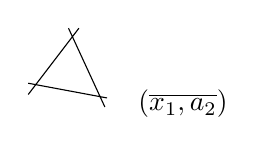
\begin{tikzpicture}[x=.55cm,y=.55cm]
 \draw (-.12,-.08)--(1.05,1.45) (.81,1.45)--(1.65,-.37) (-.12,.18)--(1.7,-.16);
 \node[anchor=west] at (2.2,-.3) {\((\overline{x_1,a_2})\)};
\end{tikzpicture}}
\[
 \underset{\substack{\Vert\\E_\gamma}}{E_{x_1}}\deleted{\simeq E_{x_2}}
\]
% archive sheet number: 116
\scanpage{116}
\diagram{\begin{tikzcd}[ampersand replacement=\&,row sep=.5em,column sep=.8em]
 \&P_3\&\\
 \&\Gamma\quad s\arrow[u]\arrow[dl]\arrow[dr]\&\\
 P_1\&\&P_2
\end{tikzcd}}
\[
 p_i(s)=a_i\qquad E=E_s\simeq E_{a_i}
\]
\[
 x_1\in P_1\qquad \gamma\longrightarrow(x_1,a_2)
\]
\diagram{\begin{tikzcd}[ampersand replacement=\&,row sep=.35em]
 E_\gamma\arrow[r,"\sim"]\arrow[d,"\unsure{2|\sim|\wr}"]\& E_{x_1}\\
 E_{a_2}\&\\
 E=E_s\arrow[u,"\sim"']\&
\end{tikzcd}}
\[
 \begin{aligned}E_{x_1}&\simeq E\\ E_{x_2}&\simeq E\\E_{x_3}&\simeq E\end{aligned}
 \qquad E_\gamma\simeq E_{p_i(\gamma)}
\]
\diagram{\begin{tikzcd}[ampersand replacement=\&,row sep=.4em,column sep=1em]
 \&\unsure{24}\& E\\
 E\&E_\gamma\arrow[l,"u"']\arrow[ur,"v"]\arrow[dr,"w"]\&\\
 \&\&E
\end{tikzcd}}
\[
 E_\gamma\longrightarrow E\quad\text{\unsure{moyennant}}
\]
\[
 \gamma\ne s\qquad {\unsure{\zeta|\xi}}_1^\gamma+\zeta_2^\gamma+\unsure{\eta_3^\gamma|\zeta_3^\gamma|\xi_3^\gamma}=0
 \qquad \gamma\longrightarrow a_1,x_2,x_3
\]
\diagram{\begin{tikzcd}[ampersand replacement=\&,row sep=.4em,column sep=.55em]
 E_{x_3}^{\deleted{\unsure{\zeta}}}\&\&\\
 \&E_\gamma\arrow[ul,"\sim"']\arrow[r,"\sim"]\arrow[d,"\sim"]\&E_{x_2}\arrow[ddl,bend left=17]\\
 \&E_{a_1}\arrow[d,"\sim"]\&\\
 \&E\&
\end{tikzcd}}
\[
 \deleted{2n^2-1}
\]
\diagram{\begin{tikzcd}[ampersand replacement=\&,row sep=.55em]
 \widetilde \Gamma\arrow[d]\\\Gamma\subset G\times G\times G
\end{tikzcd}}
\[
 \unsure{g_1+g_2+g_3=0}\qquad p_i^{-1}(a_i)
\]
\[
 \overset{\phantom{1}}{\Gamma}=
 \overset{1}{\{s\}}\ \cup\
 \overset{\overbrace{\phantom{\Gamma_1\ \cup\ \Gamma_2\ \cup\ \Gamma_3}}^{n^{\deleted{\unsure{2}}}-1}}
 {\underset{\unsure{1|i}}{\Gamma_1}\cup \Gamma_2\cup \Gamma_3}\ \cup\
 \overset{\overbrace{\phantom{\Gamma^{*}}}^{n^2-3(n-1)-1=n^2-3n+2}}
 {\overset{\unsure{\circ|o}}{\Gamma}^{*}}
\]
\[
 \Gamma_i=p_i^{-1}\{a_i\}-\{s\}
 \qquad\begin{aligned}
 \overset{\circ}{\Gamma}&=\bigcap_i p_i^{-1}(P_i-\{a_i\})\\
 &=\Gamma-\bigcup \Gamma_i-\{s\}.
 \end{aligned}
\]
\[
 \begin{aligned}
 x&\xrightarrow{\sim}y\\0&\longrightarrow y-x\\0&\longrightarrow a\\
 0&\longrightarrow b\qquad a\longrightarrow a+b
 \end{aligned}
 \qquad
 \boxed{3\mathbin{.}\deleted{\unsure{2|1}}(n-1)+2(n^2-\unsure{3|6}n+2)}
\]
\[
 \begin{aligned}
 &\deleted{\unsure{n^2\!+2|x^2\!+2}}\\
 &2n-3n+1\qquad 3n-3=3(n-1)
 \end{aligned}
\]
\[
 P_2^{*},P_3^{*},P_1^{*},\quad \Gamma^{*}\qquad
 \begin{aligned}
 vu^{-1}&=\zeta\\wu^{-1}&=\eta
 \end{aligned}
 \qquad
 \left\{\begin{aligned}uv^{-1}&=\zeta^{-1}\\wv^{-1}&=\eta\zeta^{-1}\end{aligned}\right.
\]
% archive sheet number: 117
\scanpage{117}
\[
\begin{aligned}
 g_2(\alpha_2a_1\alpha_3^{-1})g_3^{-1}&=\alpha_2a_{\unsure{2|1}}\alpha_3^{-1}\\
 (\alpha_2^{-1}g_2\alpha_2)a_1(\alpha_3^{-1}g_3\alpha_3)^{-1}&=a_1\\
 \alpha_3^{-1}g_3\alpha_3&=\widetilde a_1(\alpha_2^{-1}g_2\alpha_2)\\
 \deleted{\operatorname{int}(\alpha_2}g_3&=[\operatorname{int}(\alpha_3)\,\widetilde a_1\,\operatorname{int}(\alpha_2)^{-1}](g_2)
\end{aligned}
\]
\diagram{\begin{tikzcd}[ampersand replacement=\&,column sep=.65em,row sep=.6em]
 \&P_1\&\\
 \&\Gamma\arrow[u]\arrow[dl,dash]\&\\
 P_2\&\&P_3\arrow[ul]
\end{tikzcd}}
\[
 P_2\times P_3\ \text{---}\ P_1\quad\deleted{\times}
\]
\diagram{\begin{tikzcd}[ampersand replacement=\&,column sep=.4em,row sep=1.8em]
 G\arrow[d,"\varphi"']\&{}\times\&G\arrow[d,"\deleted{\unsure{\varphi}}\,\psi"]\arrow[r]\&G\arrow[d,"\chi"']\ \unsure{y}\\
 G_{\deleted{\unsure{1}}}\&{}\times\&G\arrow[r,dash]\&G
\end{tikzcd}}
\[
\begin{aligned}
 \varphi(x)\psi(y)&=\chi(xy).\\
 \varphi(1)=a,\quad \psi(1)&=b,\quad \chi(1)=c\\
 ab&=c
\end{aligned}
\]
\[
 \deleted{ab}\qquad\deleted{a\varphi(\unsure{x})}\qquad
 \begin{aligned}
 &\deleted{a\varphi}\qquad \varphi(x)\psi(\unsure{x|1}\\
 &\deleted{\unsure{\sigma(x)\varphi(x)}}\quad \deleted{xyz=1\Rightarrow}\\
 &\unsure{\tau.|t.}\ \varphi(\underline{x})\psi(y)\chi(z)=1\\
 &\varphi(1)\psi(1)\chi(1)=\unsure{1|d}\\
 &\underset{\deleted{\unsure{\beta}}\beta\gamma^{-1}}{\Vert}\qquad\underset{\deleted{\unsure{\alpha}}\gamma\alpha^{-1}}{|}\qquad \alpha\beta^{-1}
 \end{aligned}
\]
\[
\begin{aligned}
 &\varphi'(1)=1,\quad \psi'(1)=1,\quad \chi'(1)=1\\
 &xyz=1\Rightarrow \varphi'(x)\psi'(y)\chi'(z)=1\\
 &yz=1\Rightarrow \psi'(y)\chi'(z)=1\\
 &\chi'(z)=\psi'(y)^{-1}\\
 &\chi'(y^{-1})=\psi'(y)^{-1}\\
 &\psi'(y)=\chi'(y^{-1})^{-1}\\
 &\deleted{\unsure{\chi'}}\quad \varphi'=\psi'=\chi'\\
 &\varphi
\end{aligned}
\qquad
\begin{aligned}
 &abc=1\\
 &a=\beta\gamma^{-1}\quad b=\gamma\alpha^{-1}\\
 &\deleted{\beta\gamma^{-1}b}\quad ab\unsure{c|e|\in}=\beta\alpha^{-1}c
\end{aligned}
\]
\[
 \deleted{\unsure{\operatorname{int}\beta\,\tau_\alpha|\operatorname{int}\varphi\,\tau_{\alpha}}}
\]
\[
 \begin{array}{c|c|c}
 \tau_{\beta}^{-1}\varphi\tau_{\gamma}^{\unsure{d|*|\prime}}&
 \tau_{\gamma^{-1}}\psi\tau_{\alpha}^{\unsure{d|*|\prime}}&
 \tau_{\alpha^{\unsure{-1}}}^{\unsure{G|g}}\chi\tau_{\beta}^{\unsure{d|1|\prime}}\\
 \Vert&\Vert&\Vert\\ \varphi'&\psi'&\chi'
 \end{array}
\]
\[
 (\beta^{-1}\varphi(x)\,\underline{\gamma)(\gamma^{-1}\psi(y)\alpha)(\alpha^{-1}\chi(z)}\,\beta)=1
\]
\[
 \begin{gathered}
 (u\times u\times u)\\
 (\tau_\beta u{\tau'_\gamma}^{-1},\tau_\gamma u{\tau'_\alpha}^{-1},\tau_\alpha u{\tau'_\beta}^{-1})
 \end{gathered}
\]
% archive sheet number: 118
\scanpage{118}
\diagram{\begin{tikzcd}[ampersand replacement=\&,execute at end picture={
 \begin{scope}[x=.012cm,y=-.012cm,every node/.style={font=\scriptsize,inner sep=.5pt}]
 \coordinate (u) at (327,380); \coordinate (v) at (497,387); \coordinate (w) at (410,265);
 \draw (u)--(w)--(v)--cycle;
 \node[below right] at (u) {$u$};\node[below left] at (v) {$v$};\node[right] at (w) {$w$};
 \draw (u)--(87,314)--(79,354)--cycle (u)--(86,394)--(95,437)--cycle
       (u)--(145,501)--(166,532)--cycle (u)--(217,549)--(258,567)--cycle;
 \draw (v)--(679,311)--(677,352)--cycle (v)--(667,420)--(657,447)--cycle
       (v)--(657,504)--(635,528)--cycle (v)--(549,549)--(520,560)--cycle;
 \draw (w)--(264,168)--(290,133)--cycle (w)--(329,120)--(347,100)--cycle
       (w)--(409,100)--(445,101)--cycle (w)--(554,131)--(574,151)--cycle;
 \node[left] at (81,310) {$\alpha'_4$};\node[left] at (78,353) {$\alpha_4$};
 \node[left] at (89,391) {$\alpha'_3$};\node[left] at (94,435) {$\alpha_3$};
 \node[left] at (145,498) {$\alpha'_{\unsure{2}}$};\node[below] at (159,532) {$\alpha_2$};
 \node[left] at (217,553) {$\alpha'_1$};\node[right] at (252,570) {$\alpha_1$};
 \node at (36,332) {$a_4\big\{$};\node at (39,422) {$a_3\big\{$};
 \node at (91,551) {$a_2\big\{$};\node[below] at (218,584) {$\underbrace{\hspace{2em}}_{a_1}$};
 \node[right] at (677,311) {$\beta_1$};\node[right] at (677,347) {$\beta'_1$};
 \node[right] at (667,416) {$\beta_2$};\node[right] at (657,444) {$\beta'_2$};
 \node at (756,335) {$\big\}b_1$};\node at (770,439) {$\big\}b_2$};\node at (720,548) {$\big\}b_3$};
 \node[below] at (511,560) {$\unsure{\beta'_4|\beta'_3}$};\node[right] at (546,551) {$\unsure{\beta_4|\beta_3}$};
 \node[below] at (572,589) {$\underbrace{\hspace{2em}}_{b_4}$};
 \node[left] at (265,167) {$\gamma_1$};\node[left] at (289,131) {$\gamma'_1$};
 \node[above] at (324,121) {$\gamma_2$};\node[above] at (351,100) {$\gamma'_2$};
 \node[above] at (407,99) {$\gamma_3$};\node[above] at (455,102) {$\gamma'_3$};
 \node[above] at (556,129) {$\deleted{\unsure{\alpha}}\gamma_4$};
 \node[right] at (574,154) {$\gamma'_4$};
 \node[rotate=45] at (194,123) {$c_1\big\{$};
 \node at (337,44) {$\overbrace{\hspace{2em}}^{c_2}$};
 \node at (443,29) {$\overbrace{\hspace{2em}}^{c_3}$};\node at (681,94) {$\big\}c_4$};
 \draw[thin] (128,66)--(278,230)--(505,579);
 \end{scope}}]\phantom{.}\end{tikzcd}}
\[
 12\ \text{arêtes}\ \left\{\begin{array}{lll}
 \alpha_1,\alpha_2,\alpha_3,\alpha_4&\text{\unsure{liés|liées} à}&\beta_4\\
 \beta_1,\beta_2,\beta_3,\beta_4&\text{-------}&\gamma_4\\
 \gamma_1,\gamma_2,\gamma_3,\gamma_4&\text{-------}&\alpha_4
 \end{array}\right.
\]
\[
 \deleted{12\ \text{arêtes}\ \left\{\begin{array}{lll}
 \alpha_i&\text{lié à}&\alpha'_i\\\beta_i&\text{lié à}&\beta'_i\\\gamma_i&\text{lié à}&\gamma'_i
 \end{array}\right.\quad 1\le i\le\unsure{4|7}}
\]
\[
 12\left\{\begin{array}{ll}
 \alpha'_i\ \text{liés à}&\beta'_4\\ \beta'_i\ \text{------}&\gamma'_4\\ \gamma'_i\ \text{------}&\alpha'_4
 \end{array}\right.
\]
% margin note written sideways
\margin{\(a_1\wedge\underbrace{\unsure{x_2|a_2}\wedge\unsure{x_3|a_3}}=1\)}
\[
 \left\{\begin{array}{lll}
 \alpha_1&\text{lié à}&\beta'_1,\beta_2,\beta_3,\beta_4\\
 \alpha_2&\text{------}&\beta_1,\beta'_2,\beta_3,\beta_4\\
 \alpha_3&\text{------}&\beta_1,\beta_2,\beta'_3,\beta_4\\
 \alpha_4&\text{------}&\beta'_1,\beta'_2,\beta'_3,\beta_4
 \end{array}\right.
 \quad
 \begin{gathered}\alpha'_1\ \text{lié à}\ \beta_1,\beta'_2,\beta'_3,\beta'_4\\\text{----}\end{gathered}
\]
% margin note written sideways
\margin{\({}_{G_2}P_1\underset{G_3}{\wedge}(\unsure{U}P_2\underset{G_3}{\wedge}P_3)_{G_2}\)}
\[
 \boxed{\begin{aligned}\alpha_1&\text{ lié à }\beta'_1\\ \alpha_{\unsure{1|2}}&\text{ lié à }\beta_2\end{aligned}}
 \quad\underset{\longleftarrow}{\boxed{\alpha_1\text{ lié à }\gamma'_4}}
 \quad
 \begin{aligned}
 \alpha_{\unsure{3|1}}&\text{ lié à }\deleted{\unsure{\gamma}}\beta_4\text{ et }\gamma'_4\\
 \beta_1&\text{ lié à }\gamma_4\text{ et }\beta'_4\\
 (\alpha_1&\text{ lié à }\beta_1)\Rightarrow\\
 \alpha_1&\text{lié}
 \end{aligned}
\]
\diagram{\begin{tikzcd}[ampersand replacement=\&,row sep=.8em,column sep=.6em]
 \&\&w\&\&\\
 \&u\arrow[ur]\arrow[rr,dash]\arrow[dl,dash]\arrow[d,dash]\&\&v\arrow[ul,dash]\arrow[d,dash]\arrow[dr,dash]\arrow[drr,dash]\&\&\\
 \unsure{\alpha|v}\&\unsure{\alpha'|\alpha_2}\&\&\beta\&\beta'\&\beta''\\
 {\Vert}\&{\Vert}\&\&{\Vert}\&{\Vert}\&\\
 \unsure{\alpha_1|\alpha}\&\alpha'_2\&\&\beta'_1\&\beta_2\&
\end{tikzcd}}
\[
 \left\{\begin{array}{lll}
 \alpha_1&\beta'_1,&\gamma'_4\\\alpha_1,&\beta_2,&\gamma_{\unsure{2|3}}\\
 \alpha'_2,&\beta'_1,&\gamma'_3\\\alpha'_2,&\beta_2,&\gamma_4
 \end{array}\right.
\]
% margin note written sideways; group calculations run upwards from the right edge.
\[
\begin{aligned}
 &\deleted{g_2a_1g_3^{-1}=1}\\
 &g_2(\alpha_2a_1\alpha_3^{-1})g_3^{-1}=\alpha_2a_1\alpha_3\\
 &(g_2\alpha_2)a_1(\deleted{\unsure{\alpha}}g_3\alpha_3)^{-1}=\alpha_2a_1\alpha_3\\
 &g_3\alpha_3=\widetilde a_1(g_2\alpha_2)\\
 &\widetilde a_1(g_2)\widetilde a_1(\alpha_2)\unsure{'|,}=g_3\alpha_3\\
 &g_3=\\
 &\widetilde A_1(g_2)\alpha_3=\widetilde a_1(g_2)\deleted{\unsure{\alpha}}\widetilde a_1(\alpha_2)\\
 &\widetilde A_1(g_2)=\widetilde a_1(g_2)\widetilde a_1(\alpha_2)\alpha_3^{-1}
\end{aligned}
\]
\figure{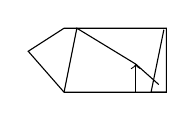
\begin{tikzpicture}[x=.65cm,y=.65cm]
 \draw (0,0)--(-.7,.8)--(0,1.25)--(2,1.25)--(2,0)--cycle;
 \draw (0,0)--(.25,1.25)--(1.4,.55)--(1.85,.15);
 \draw[->] (1.4,0)--(1.4,.55);
 \draw (1.7,0)--(1.95,1.22) (1.7,0)--(2,0);
\end{tikzpicture}}
% Lower-edge text is inverted relative to the large graph.
\[
\begin{aligned}
 &g_2a_1=a_1g_3\deleted{=b_1}&&\text{i.e. }g_2a_1g_3^{-1}=a_1\\
 &g_3a_2=a_2g_1=b_2&&\text{i.e. }g_3a_2g_1^{-1}=a_2\\
 ?\ \Downarrow\quad&g_1a_3=a_3g_2&&a_1,a_2,
\end{aligned}
\]
\[
 \underbrace{(g_1,g_2,g_3)\underbrace{(a_1,a_2,a_3)}_{\in \Gamma}}_{\in \Gamma}
       =(a_1,a_2,\unsure{a_3|a'_3})
\]
% archive sheet number: 119
\scanpage{119}
\[
\begin{aligned}
 &\deleted{u\in\operatorname{Aut}G}\\
 &\tau_\beta u\tau'_{\gamma^{-1}}\quad \tau_{\gamma'}u'\tau'_{\gamma'}{}^{-1}\\
 &\deleted{\beta u(x)\gamma^{-1}}\quad u'(x{\gamma'}^{-1})\\
 &\beta u(x\gamma^{-1})\\
 &\beta'u'(\deleted{\unsure{\gamma}}\beta u(x\gamma^{-1}){\gamma'}^{-1})\\
 &\beta'u'(\beta)\,\underline{u'u}(x)
\end{aligned}\qquad
\begin{aligned}
 \varphi(1)&=\beta\gamma^{-1}\\
 \varphi'(x)&=\beta^{-1}\varphi(x)\gamma^{\deleted{\unsure{-1}}}\\
 \deleted{\varphi}\psi'(x)&=\gamma^{-1}\psi(\unsure{z|x})\deleted{\unsure{\beta}}\alpha\\
 \chi'(x)&=\deleted{\unsure{\beta}}\alpha^{-1}\chi(x)\beta\\
 \varphi'(\unsure{a|x})\unsure{\psi'|\psi}(\unsure{b|y|x})\chi'(\unsure{c|z|x})&=0\\
 \varphi&=\beta u(x)\gamma^{-1}
\end{aligned}
\]
\[
 \begin{gathered}
 \operatorname{Aut}(G)\\G\times G\\
 \deleted{(u,\beta,\gamma,\beta}\quad\deleted{u,\beta,}
 \end{gathered}
 \qquad \deleted{u(x\gamma^{-1})}
\]
\[
 (u,\alpha,\beta,\gamma)(x,y,z)=
\]
\diagram{\begin{tikzcd}[ampersand replacement=\&,row sep=.65em,column sep=1.5em]
 \&{\overset{u}{\tau_\beta}\tau'_{\deleted{\unsure{\alpha}}\gamma}u^{\deleted{\unsure{*}}}}\\
 {(u,\alpha,\beta,\gamma)}\arrow[ur]\arrow[r]\arrow[dr]\&{\tau_\gamma\tau'_{\deleted{\unsure{\beta}}\alpha}u}\\
 \&{\tau_{\unsure{\alpha|2}}\tau'_\beta u}
\end{tikzcd}}
\[
 \begin{aligned}
 &(\tau_\beta\tau'_\gamma u)(\tau_{\beta'}\tau'_{\gamma'}u')\\
 &\beta u(x)\gamma^{-1}=x\\
 &\beta=\gamma
 \end{aligned}
\]
\[
\begin{aligned}
 &\deleted{\unsure{\beta\gamma}}\beta u(\beta'u'(x){\gamma'}^{-1})\gamma^{-1}=\\
 &\hspace{2em}\beta u(\beta')uu'(x)\bigl(\gamma u(\gamma')\bigr)^{-1}\\
 &\hspace{18em}u(\alpha')=\alpha^{-1}\\
 &\hspace{18em}\alpha'=u^{-1}(\alpha^{-1})
\end{aligned}
\]
\[
\begin{aligned}
 &(u,\alpha,\beta,\gamma)(u',\alpha',\beta',\gamma')=(uu',\alpha u(\alpha'),\beta u(\beta'),\gamma u(\gamma')\\
 &\bigl((u,\alpha,\beta,\gamma)\,(u',\alpha',\beta',\gamma')\bigr)(u'',\alpha'',\beta'',\gamma'')
 \unsure{\mathbin{:}|=}\bigl(uu'u'',\alpha u(\alpha')uu'(\alpha''),\text{---}\bigr)\\
 &\hspace{6em}\bigl(\underbrace{\hspace{6em}}_{u'u'',\,\alpha'u'(\alpha'')\,\text{---}}\bigr)
 \qquad\bigl(u\,u'u'',\,\alpha u(\alpha'u'(\alpha''))\\
 &(u,\alpha,\beta,\gamma)(u^{-1},u^{-1}(\alpha)^{-1},u^{-1}(\beta)^{-1},u^{-1}(\gamma^{-1})
\end{aligned}
\]
% archive sheet number: 120
\scanpage{120}
% Writing on ruled music paper. Turn the archive image through 180 degrees.
% archive sheet number: 121
\figure{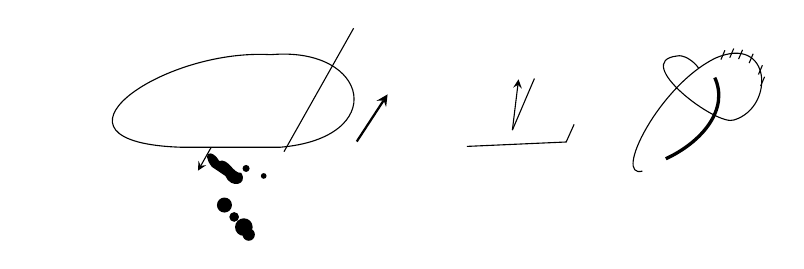
\begin{tikzpicture}[scale=.56,>=stealth]
\draw (0,0) .. controls (-3.5,.1) and (-.5,2.25) .. (2,2.1) .. controls (4.25,2.3) and (4.7,.2) .. (2.2,0) -- cycle;
\draw[->,thick] (3.95,.13)--(4.65,1.2); \draw[->] (.65,0)--(.35,-.53);
\draw (2.3,-.1)--(3.88,2.7);
\draw (6.45,.02)--(8.7,.12)--(8.88,.52); \draw[->] (7.48,.39)--(7.62,1.54); \draw (7.48,.39)--(7.98,1.56);
\draw (10.43,-.54).. controls (9.75,-.72) and (10.8,1.39)..(12.08,2.02)..controls(13.36,2.58)and(13.44,.91)..(12.51,.62)..controls(12.12,.46)and(10.16,1.95)..(11.21,2.07)..controls(11.36,2.11)and(11.59,1.96)..(11.7,1.8);
\draw[very thick] (10.96,-.26)..controls(11.78,.12)and(12.4,.86)..(12.07,1.58);
\foreach \x/\y in {12.25/2.08,12.45/2.12,12.65/2.09,12.89/2.0,13.1/1.74,13.15/1.48}{\draw (\x-.04,\y-.09)--(\x+.05,\y+.12);}
\fill (.66,-.44) ..controls(.4,-.09)and(.69,-.04)..(.83,-.31)..controls(1.05,-.24)and(1.14,-.6)..(1.33,-.58)..controls(1.5,-.85)and(1.09,-.95)..(.97,-.65)--cycle;
\foreach \x/\y/\r in {1.44/-.48/.08,1.84/-.65/.065,.95/-1.31/.17,1.17/-1.58/.11,1.39/-1.81/.2,1.5/-1.98/.14}{\fill (\x,\y) circle (\r);}
\end{tikzpicture}}
\[
\deleted{\unsure{P|p}}\quad \Gamma\longrightarrow S^1
\]
\[
 S^2\times S^2-\mathrm{diag}\qquad
 {\displaystyle S^2\times S^2/\mathord{\pm}1}\ \deleted{\unsure{-|/}}\Delta
\]
\diagram{\begin{tikzcd}[ampersand replacement=\&,column sep=.55em]
 {}\&{}\&\pi_1(S^1)=\mathbb Z\arrow[d,"2"']\\
 {}\&{\unsure{\mathbb C|C}}^{*}\arrow[d]\&\pi_1(C^{\unsure{*|1}})=\mathbb Z\arrow[d]\\
 {\deleted{S^2\times S^2-\mathrm{diag}-\unsure{\mathrm{antidiag}|\mathrm{antid}}} =}\&\unsure{\mathbb P|P}\arrow[d]\&\pi_1(\unsure{\mathbb P|P})\arrow[d]\\
 S^1\arrow[r]\&S^2\&\pi_1(S^2)=0
\end{tikzcd}}
\[
 (x,y)\qquad\begin{array}{l}\deleted{\unsure{y}=x}\\ y=-x\end{array}
\]
\figure{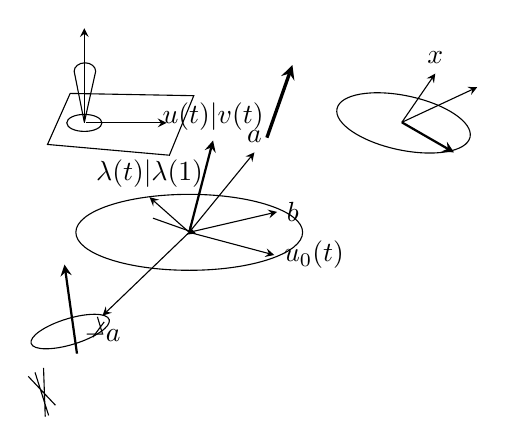
\begin{tikzpicture}[scale=.72,>=stealth]
\draw (-2.1,1.55)--(-2.5,.65)--(-.35,.46)--(.08,1.51)--cycle;
\draw (-1.85,1.03) ellipse (.31 and .15); \draw (-1.85,1.04)--(-2.03,1.94) arc[start angle=180,end angle=0,x radius=.19,y radius=.15]--(-1.85,1.04);
\draw[->] (-1.85,1.03)--(-1.85,2.7);\draw[->](-1.82,1.03)--(-.4,1.03);
\draw (0,-.9) ellipse (2 and .67);
\draw[->] (0,-.9)--(-.7,-.28) node[above]{$\unsure{\lambda(t)|\lambda(1)}$};
\draw[->,thick] (0,-.9)--(.42,.72) node[above]{$\unsure{u(t)|v(t)}$};
\draw[->] (0,-.9)--(1.15,.51) node[above]{$a$};
\draw[->] (0,-.9)--(1.55,-.54) node[right]{$b$};
\draw[->] (0,-.9)--(1.5,-1.3) node[right]{$u_0(t)$};
\draw[->] (0,-.9)--(-1.53,-2.37) node[below]{$-a$};
\draw[->,very thick] (1.37,.77)--(1.82,2.05); \draw[->] (-.64,-.65)--(.12,-.92);
\draw (-2.1,-2.65) ellipse[x radius=.72,y radius=.23,rotate=17]; \draw[->,thick](-1.98,-3.04)--(-2.2,-1.47);
\draw (-1.5,-2.48)--(-1.7,-2.75) (-1.62,-2.39)--(-1.53,-2.69);
\draw (-2.72,-3.37)--(-2.48,-4.13) (-2.84,-3.44)--(-2.36,-3.95) (-2.57,-3.29)--(-2.54,-4.15);
\draw (3.78,1.03) ellipse[x radius=1.2,y radius=.48,rotate=-12];
\draw[->] (3.75,1.04)--(4.34,1.9)node[above]{$x$};
\draw[->] (3.75,1.04)--(5.08,1.66);
\draw[->,thick] (3.75,1.04)--(4.67,.51);
\end{tikzpicture}}
\[
 \unsure{\theta|\Theta}(t): S^1\longrightarrow S^2 \qquad
 \deleted{{\unsure{P|p|\mathbb P}}^1\times P^1-P^1}
\]
\diagram{\begin{tikzcd}[ampersand replacement=\&,row sep=small]
 {}\&{}\& L\\
 X\times\&E\arrow[ur]\arrow[dr]\&{}\\
 F\arrow[ur,dash]\arrow[rr,"\sim"']\&{}\& L'
\end{tikzcd}}
\[
 \underline{1\text{-}\mathrm{hom}}\,(\unsure{h|u|L},F)\qquad E\simeq L\oplus L'
 \qquad \boxed{p^2=p\quad\mathrm{Tr}\,p=1}
\]
\[
 0\longrightarrow F\longrightarrow E_p\longrightarrow\underline{\mathcal O}(1)\longrightarrow0
\]
\[
 F\oplus\mathcal O(1)\simeq \unsure{\mathcal O|0}\qquad
 F\simeq\mathcal O(-1)\qquad \underline{\mathcal O}(-2)
\]
\figure{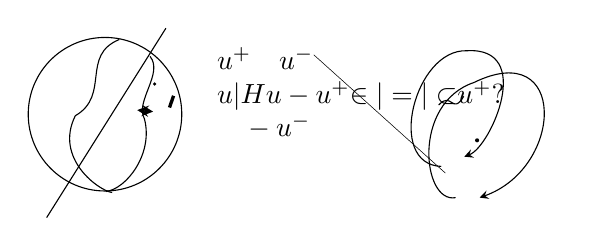
\begin{tikzpicture}[scale=.65,>=stealth]
\draw (0,0) circle (1.5); \draw (.28,1.46) .. controls(-.48,1.15)and(.11,.37)..(-.58,-.03)..controls(-1,-.87)and(-.11,-1.5)..(.14,-1.53);
\draw (.88,1.13)..controls(1.15,.8)and(.58,.25)..(.77,-.09)..controls(.95,-.77)and(.42,-1.46)..(.02,-1.51);
\draw[<->,thick] (.63,.08)--(.94,.05); \fill (.97,.59) circle (.035); \draw[very thick] (1.26,.13)--(1.34,.36);
\draw (-1.14,-2.02)--(1.19,1.68);
\node[anchor=west,align=left] at (2,.41){$u^+\quad u^-$\\$\deleted{\unsure{u|H}}u-u^+\unsure{\in|=|\subset}u^+?$\\$\phantom{u}\ -u^-$};
\draw[very thin] (4.08,1.16)--(6.65,-1.15);
\draw[->] (6.57,-1.02)..controls(5.48,-.98)and(6.05,1.28)..(7.07,1.24)..controls(8.4,1.32)and(7.54,-.63)..(7.02,-.83);
\draw[->] (6.85,-1.63)..controls(6.2,-1.75)and(5.99,.21)..(7.21,.62)..controls(9.04,1.51)and(8.97,-1.04)..(7.32,-1.63);
\fill (7.27,-.51) circle (.04);
\draw (6.52,.18) .. controls (6.78,.46)and(6.78,-.03).. (7.01,.35);
\end{tikzpicture}}
\figure{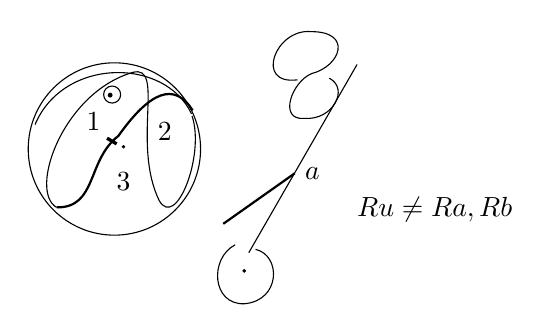
\begin{tikzpicture}[scale=.72,>=stealth]
\draw (0,0) circle (1.52); \draw (-1.4,.43)..controls(-.9,1.62)and(.89,1.62)..(1.36,.62);
\draw (-1.02,-1.03)..controls(-1.52,-.74)and(-.91,.99)..(.32,1.35)..controls(.9,1.51)and(.3,.1)..(.79,-.91)..controls(1.09,-1.43)and(1.6,-.1)..(1.37,.58);
\draw[thick](-1.02,-1.03)..controls(-.3,-1.04)and(-.49,-.2)..(.07,.23)..controls(.63,1.02)and(1.06,1.19)..(1.38,.68);
\draw (-.04,.96) circle(.15); \fill (-.075,.95) circle(.043); \draw[very thick](-.13,.19)--(.04,.09); \fill(.16,.04)circle(.034);
\node at(-.37,.49){$1$};\node at(.89,.31){$2$};\node at(.16,-.58){$3$};
\draw (3.23,1.22)..controls(2.46,1.12)and(2.84,2.13)..(3.47,2.07)..controls(4.21,2.07)and(3.99,1.46)..(3.48,1.33)..controls(3.13,1.19)and(2.88,.5)..(3.35,.54)..controls(3.85,.5)and(4.15,1.06)..(3.79,1.25);
\draw[thick] (1.92,-1.32)--(3.18,-.43)node[right]{$a$};
\draw (2.13,-1.69)..controls(1.67,-1.93)and(1.72,-2.75)..(2.29,-2.73)..controls(2.93,-2.68)and(2.95,-1.88)..(2.49,-1.77);
\fill (2.29,-2.15) circle(.035); \draw[thin] (2.37,-1.83)--(4.28,1.49);
\node at(5.65,-1.07){$\mathbb R u\ne\mathbb R a,\mathbb R b$};
\end{tikzpicture}}
% crop-candidate: scan 120
